\documentclass{report}[12pt]
\usepackage{amsmath}
\usepackage{graphicx}
\usepackage{float}
\usepackage{amssymb}
\usepackage{import}
\usepackage{tikz}
\usepackage{booktabs}
\usepackage{mathtools}
\graphicspath{{Imagens/}}
\author{}
\date{}
\begin{document}
\chapter{Estudos Iniciais}
\section{Ideias e outras coisas}
(Qual a possibilidade de conseguirmos fazer uma regressão, por exemplo, e irmos estimando e atualizando
os parametros por meio da informação de fisher?)
Estava pesquisando sobre as limitações e achei interessante o artigo 'Notes on the Limitations of the Empirical Fisher Approximation'
no qual ele delimita algumas coisas quanto o calculo e aproximações da informação de fisher, em principal
quanto seu não uso por falta de um método conveniente para que seja usado, principalmente na area de
deep learning. Ademais uma boa aproximação para que seja calculado, com certo grau de precisão e utilidade
aparentemente se falta. Eles mostram que enquanto pode ser calculado muitas vezes o valor bruto até 
rapidamente, quem sabe uma aproximação não seja util, ou talvez tentar traze-lo para o mundo dos computadores
com um maior peso.\par

Kullback–Leibler divergence/Hellinger distance


\section{Informação de Fisher}
Inicialmente, vamos imaginar a seguinte situação: Eu lhe dou um grafico de uma distribuição normal,
onde você não sabe onde ela esta centrada, porem sabe qual sua variancia. A partir do grafico dela,
voce conseguiria deduzir, ou talvez obter alguma informação sobre o valor real de $\mu ^{\star}$?
Observe às seguintes curvas e tente achar suas medias
\begin{figure*}[ht]
    \centering    
        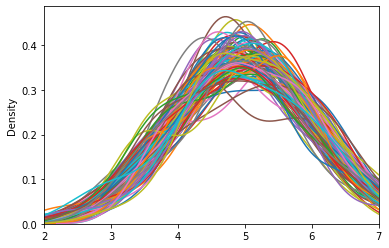
\includegraphics[scale=0.4]{normal 51.png}
        \caption{Normal com variância 1}
        \label{fig:Normal 51}
\end{figure*}
\begin{figure*}[ht]
    \centering    
        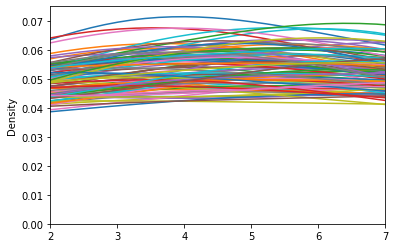
\includegraphics[scale=0.4]{normal 57.png}
        \caption{Normal com variância 7}
        \label{fig:Normal 57}
\end{figure*}
Em uma é muito mais facil identificar onde possivelmente o valor \(\mu ^{\star}\) está, mas digamos
que precisamos saber o da segunda distribuição e em um caso mais geral, para qualquer distribuição.
Que valor poderiamos tentar atribuir a quantidade de informações que podemos tirar de uma base de dados?
A definição da informação de fisher, em dados matematicos é dado por
\begin{equation}
    \mathcal{I} _{X}(\theta)= \begin{dcases}
        \sum_{x \epsilon \chi}(\frac{\mathrm{d}}{\mathrm{d}\theta } \log f(x|\theta))^{2}p_{\theta } (x)  , &\text{se X não é continuo   }  ;\\
        \int_{\chi}(\frac{\mathrm{d}}{\mathrm{d}\theta } \log f(x|\theta))^{2}p_{\theta } (x)\mathrm{d}x, &\text{se X é continuo }  ;\\
    \end{dcases} 
\end{equation}
O valor \(\frac{\mathrm{d}}{\mathrm{d}\theta } \log f(x|\theta )\) é conhecido como a função score,
que descreve quão sensitivo é o modelo a uma mudança no \(\theta \) em um \(\theta \) particular. A
informação de fisher mede a sensitividade da relação entre \(f\) e mudanças no \( \theta \) pesando na
a sensitividade a cada valor de \(x\) em respeito a probabilidade definida por \(p_{\theta } f(x|\theta )\) 
Esse peso em relação a \( p(\theta )\) faz com que a informação de fisher seja em relação ao valor
esperado de \(\theta \). Podemos definir a inforção de fisher em relação a esperança.
Vamos assumir algumas coisas para depois conferirmos se estamos corretos. Numa normal, sua variancia
não pode ser zero, mas quanto mais perto de zero estivermos, maior a informação que vamos ter.
Quanto maior nossa variancia, menor a quantidade de informações que vamos conseguir tirar do nosso parametro.
Se nosso modelo seguir isso, estamos no caminho certo
\begin{equation} \scriptstyle
    \mathcal{I} _X(\theta)=-E(\frac{\mathrm{d^{2}}}{\mathrm{d}x^{2} } \log f(x|\theta ))=
    \begin{dcases} 
        \scriptstyle-\sum_{x \epsilon \chi}(\frac{\mathrm{d^{2} }}{\mathrm{d}\theta^{2}  } \log f(x|\theta))^{2}p_{\theta } (x),&\text{\small se X não é continuo };\\
        \scriptstyle-\int_{\chi}(\frac{\mathrm{d^{2} }}{\mathrm{d}\theta^{2}  } \log f(x|\theta))^{2}p_{\theta } (x)\mathrm{d}x,&\text{\small se X é continuo };\\
    \end{dcases}
\end{equation}
Vamos fazer um exemplo para a Normal.
\begin{gather*}
    \intertext{Sabendo que a equação de uma normal é dada por}\\
    N(\mu,\sigma^{2} )=\frac{1}{\sqrt{2\pi \sigma ^{2}  } } \exp ^{\frac{(x-\mu )^{2}}{2\sigma ^{2} }}\\
    \intertext{sua função logaritmo é dado por} \\
    l(\theta)=-\frac{1}{2}\ln (\sigma ^{2}  )-\frac{(x-\mu )^{2}}{2\sigma ^{2} }+c\\
    \intertext{Como ja temos \(\sigma \), nosso \(\theta \) onde queremos obter informaçã é o \(\mu \) } 
    \intertext{Logo, colocando \(\mu =\theta \) e achando nossas funções} \\
    l^\prime_{\theta  }  (\theta)=\frac{x-\theta  }{\sigma^{2} }\\
    l^{\prime \prime }_{\theta} (\theta)=-\frac{1}{\sigma^{2} }\\
    \intertext{Fazendo a esperança, temos}\\
    -E(l^{\prime \prime }_{\theta } (\theta))=\frac{1}{\sigma ^{2} }\\
\end{gather*}
Então ela depende apenas da variancia da nossa distribuição. Se observamos os graficos \ref*{fig:Normal 51}
e \ref*{fig:Normal 57}, observamos que na primeira é mais facil tentar assumir o valor de \(\mu \) enquanto
na segunda não tanto. Isso condiz com o comportamento do grafico e seus respectivos valores de variancia.
Então essa nossa discussão foi feita corretamente
\begin{figure*}[ht]
    \centering    
        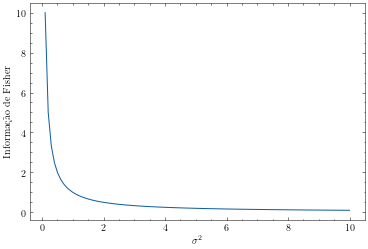
\includegraphics[scale=0.8]{informação de fisher normal.png}
        \caption{Infomação de Fisher por Sigma}
        \label{fig:Info_fish_normal}
\end{figure*}
\section{Informação de Fisher e Flips ecologicos (Artigo original)}
\subsection{Método e equações}
Um dos pontos principais em que precisamos nos apoiar é a ideia de que em sistemas que estão proximos
ou em um regime dinamico estatico, possuem valores de variabilidades fixos em suas variaveis de estados
e qualquer mudança no sistema é manifestada por meio de mudança nas variabilidades. Ou seja,
se tivermos um vetor de variaveis dados por
\begin{gather*}
    \mathbf{X} =
    \begin{pmatrix}
        x_ 1 & x_ 2 & \ldots  &  x_ n \\
    \end{pmatrix}\\
    \mathbf{\Sigma}=  
    \begin{pmatrix}
        \sigma _1 & \sigma _2 & \ldots  &  \sigma _n \\
    \end{pmatrix}
\end{gather*}
Onde \(\mathbf{X} \) é o vetor contendo todos as variaveis do regime e \(\mathbf{\Sigma} \) é o vetor
contendo todas suas variabilidades, com valores iguais a \(\sigma _1,\sigma _2,\ldots ,\sigma _n\).
Se o regime fosse estados, esses valores se materiam constantes, ou em um padrão. Caso ele esteja mudando
os valores de \(\sigma \) mudariam tambem. Dado isso, vamos aplicar a informação de fisher. Utilizando
a formula:
\begin{equation}
    I=\int \frac{1}{p(\varepsilon )}(\frac{\mathrm{d}p(\varepsilon )}{\mathrm{d}\varepsilon  })^{2} \mathrm{d} \varepsilon
\end{equation}
 
Aonde \(p(\varepsilon )\) é a distribuição de probabilidades do erro,distancia \(\varepsilon \) do valor real.
Assumindo que o sistema pode ser descrito como dinamico continuo e está num ciclo periodico estavel, podemos
definir a informação de fisher, depois de uma certa quantia de matematica (fazer isso depois, Marco.), Como:
\begin{equation}
    I=\frac{1}{T}\int_{0}^{T} \frac{(R^{\prime \prime }(t))^{2} }{(R^\prime (t))^4} \,\mathrm{d}t 
\end{equation}
Isso para apenas um ciclo do sistema. Na forma vetorial
\begin{equation}
    I=\frac{1}{T}\int_{0}^{T} \frac{(\mathbf{x}^\prime(t))^T (\mathbf{x}^{\prime \prime}(t))^{2} }{\lVert \mathbf{x^\prime } (t) \rVert ^6} \,\mathrm{d}t
\end{equation}
    
Fazendo uma interpretação. Sendo \(\mathbf{x}^\prime  (t)\) a velocidade do nosso sistema e  similarmente
\(\mathbf{x}^{\prime \prime }(t)\)  como a aceleração do sistema e pelo nosso desenvolvimento de como chegamos
nela em primeiro lugar, estamos medindo a variabilidade do nosso sistema durante o tempo que ele passa
em cada seção da sua trajetoria. Pode ser visto tambem como a mudança de velocidade ao longo da trajetoria.
Em um sistema de velocidade 0, teriamos uma informação infinita, pois qualquer ponto que pegarmos, 
ele contera todas as informações, pois ele só teria o mesmo estado. Num sistema sem aceleração, de velocidade constante, nossa informação é
0, pois se fossemos olhar um ponto da trajetorio no ciclo 0 e no ciclo 1, estariamos vendo o mesmo estado
nos dois ciclos. Para avaliarmos nossa expressão, uma solução analitica é inviavel, numa grande
parcela das vezes. \par
Podemos, então, nos voltar para uma solução numerica que nos dará uma boa solução. A primeira coisa
que precisamos fazer é uma estimativa da velocidade e da aceleração do sistema. Como muitas vezes
o intervalo de tempo entre a coleta de dados, no mundo real, não está em intervalos regulares, podemos
continuar com esses intervalos irregulares, ou podemos interpolar para acharmos dados que são lineares.
A estimativa é feita usando 3 pontos, onde escolhemos um que é central, um a uma distancia \(\Delta t_p\) 
e a distancia \(\Delta t_a\), pela formula \(t-\Delta t_p\) e \(t\Delta t_a\) e esses intervalos estão
relacionados por \(\frac{\Delta t_a}{\Delta t_b}=\alpha \). Pela nossa definição de derivada, temos
\begin{equation}
    \mathbf{f^\prime }(t)=\frac{\alpha^{2} \mathbf{f} (t+\Delta t_a)-(\alpha ^{2} -1)\mathbf{f}(t)-\mathbf{f} (t-\alpha \Delta t_a)}{(\alpha ^{2} +\alpha )\Delta t_a} 
\end{equation}
e aceleração
\begin{equation}
    \mathbf{f} ^{(\prime \prime)}=\frac{\alpha \mathbf{f} (t+\Delta t_a)+\mathbf{f} (t-\alpha \Delta t_a)-(\alpha +1)\mathbf{f} (t)}{(\alpha ^{2} +\alpha )\Delta t_{a}^{2} /2 }
\end{equation}
\subsection{Discussão e interpretação do modelo}
Essas estimativas podem gerar alguma especie de barulho e outros dados. Um jeito de arrumar isso é 
usando uma média de dois pontos, inves de necessariamente apenas dos valores calculados. Mas o proprio
calculo de fisher já da uma ajuda em relação a isso. Ademais, não sabemos a peridiciocidade do nosso
sistema, e quando não sabemos isso, nossa informação vai ficar flutuando entre os calculos. Para isso
podemos fazer uma estimativa do periodo do sistema, utilizando uma FFT, ou conhecimentos previos. Mas
a informação de fisher é muito sensitiva se o sistema não esta em forma periodica, ou está sobre ações
de outras forças ela vai flutuar. Podemos claro aplicar a sistemas não periodicos, mas sua interepretação
sera dificil (Sera que isso ainda é verdade? Pesquisar depois). \par
Para observamos a transição, podemos simplesmete avaliar a integral em um periodo, colocando o valor como o valor do periodo todo. Isso
da uma estimativa grosseira, digamos assim, onde ela vem, geralmente, em formato de blocos. Ou podemos
fazer uma quase convolução, onde fazer a média movel, colocando o valor da integral como um unico ponto
no espaço, onde a informação de fisher usa uma janela de tamanho equivalente ao periodo, centrada no
ponto, posteriormente mudando nossa janela para o proximo ponto e assim sucessivamente. Os resultados
realmente mostram uma mudança na informação de fisher entre um periodo e outro, então é sim um
método válido. \par
(Não sei dizer se necessariamente é quando muda a informação e como eles definem ser transição ou quando
ele muda pra outro estado ciclo, talvez seja algo em relação a ecologia, ou já seja algo definido
e na aplicação real a gente so conseguiria definir que esta mudando, sem necessariamente saber se esta
indo para transição ou para outro estavel.)
\subsection{Conclusões finais}
Alguns pontos importantes a serem reforçados é que por mais que sejam uteis, a pesquisa ainda estão
incompletas (isso é so uma preliminar do primeiro artigo, posteriormente adicionarei sobre novas biografias).
Um dos pontos que precisam ser estudados é a regularização do intervalo de integração da informação, pois
diferenças nesses tempos podem levar a graficos que são de dificil interpretação. Ademais, para sistemas
aciclicos, não é de muita utlidade esse informação, pois ela variaria muito. Para sistemas muitos complexos,
com muitas variaveis, ainda é meio dificil e não tão bom. Geralmente ela se da melhor com escalas temporais
e sistemas um pouco menos complexos. O valor em si da informação ainda não é muito bem definido, valores
altos indicam um sistema mais estavel, porem valores proximos necessariamente indicariam regimes parecidos,
ou apenas com variabilidades parecidas? Quantas variaveis deveriamos considerar? Para escalas de tempo
pequenas, ainda vamos conseguir usar isso para detectar? A informação ainda é extremamente sensitiva
a forças internas, qualquer pertubação e casos em que não necessariamente é ciclico, já existe algum
modelo que seja mais robusto a isso? Claramente a informação é muito util, porem é preciso ver seu
desenvolvimento.
\chapter{Importancia}
Mais do que nunca no mundo vem se falando sobre a importancia dos nossos sistemas ecologicos. É
inegavel o profundo impacto que fizemos no planeta, principalmente nos ultimos anos e agora estamos
começando a lidar com as consequencias. Não é segredo que alteramos muito a ordem natural dos
ecossistemas, seja de forma negativa ou de forma positiva. imaginando a situação em que queremos
recuperar um certa área que foi afetada, seria muito util termos uma métrica ou uma ideia de se está
funcionando, se o que está sendo feito está realmente sendo util. Claro que, teoricamente, apenas
visualmente poderiamos tentar imaginar, mas algo que seja mais certeiro é desejado. Se selecionarmos
uma certa quantia de variaveis, como por exemplo, tamanho populacional de uma certa especie,
quantidade de um certo nutriente no solo, massa de liquens nas arvores, dentre outras, uma métrica
que pudesse avaliar a evolução das variaveis com o tempo e que nos dissese com um numero, ou algo
similar, que a evolução está acontecendo seria de grande ajuda. \par

Identificação de mudanças em sistemas ecologicos tem algo que tem crescido muito nos ultimos e o uso
de estatistica, principalmente na sua forma mais moderna, pode se tornar algo fundamental para essa
área.(pensar em algo pra escrever melhor. Não muito bom)
\chapter{Uma analise profunda da informação de Fisher}
\section{Um passo para trás}
Eu acho que é importante para realmente entender e fazer as corretas derivações necessarias, ter o
conhecimento de infomações que precedem o nosso objetivo final, tanto para realmente entender, não
so copiar uma formula, tanto para entender de onde possivelmente são os erros e possiveis locais de
melhoria. Então por enquanto, farei uma pesquisa sobre as materias que levam à informação de fisher.
\subsection{Estatistica suficiente}
Colocando que temos um conjunto de dados \(X_1,X_2,\ldots ,X_n\) gerados por uma função de
probabilidade qualquer com parametro \(\theta \), se existir uma estatistica
\(Y=u(X_1,X_2,\ldots,X_n)\), tal que a condicional \(P(X_1,X_2,\ldots ,X_n|Y=y)\) não depender de
\(\theta \). Exemplo: \par
Dado uma distribuição de bernoulli, com parametro \(\theta \) desconhecido, onde se fazem n testes
tal que existam n dados. Uma estatistica suficiente para esse parametro é a soma de todos os
\(X_i\), pois:
\begin{align*}
    Y=\sum_{i} X_i \\
    P(X_1,X_2,\ldots ,X_n|Y=y)&=\frac{p(X_1=x_1,X_2=x_2,\ldots ,X_n=x_n,Y=y)}{P(Y=y)}\\
    &=\frac{P(X_1=x_1,X_2=x_2,\ldots ,X_n=x_n,\sum_{i} X_i=x_i)}{P(\sum_{i} X_i=x_i)}
\end{align*}
Não dependendo do parametro \(\theta\). Ou seja, conseguimos toda informação possivel sobre o
parametro, apenas com essa estatistica, pois independente dele, adicionando, retirando dados,
nenhuma informação a mais sobre o parametro será ganhada. \par

Infelizmente, essa condição não nos da o necessario para calcularmos que estatistica será essa,
então ainda é um grande de um trabalho imaginarmos isso. Por sorte, temos um teorema que nos ajudará
nesse quesito, o \textit{Teorema da Fatorização} em que ele fala que se uma estatistica
\(Y=u(X_1,X_2,\ldots ,X_n)\), so é suficiente se e apenas se, a distribuição
\(f(x_1,x_2,\ldots,x_n;\theta )\), que gerou dos dados, pode ser fatorizada em dois fatores,
\(\phi,h \), da forma \(f(x_1,x_2,\ldots,x_n;\theta )=\phi
(u(x_1,x_2,\ldots,x_n);\theta)h(x_1,x_2,\ldots,x_n)\), onde \(\phi\) que é dependente dos dados
apenas por meio de \(u(x_1,x_2,\ldots,x_n)\) e \(h\) é independente do parametro. Vamos à um
exemplo:
Suponha uma bernoulli de parametro \(\theta \) desconhecido e constante. Coletando n dados de forma
independente, podemos achar nossa estatistica de modo
\begin{align*}
    f(x_1,x_2,\ldots ,x_n;\theta)&=f(x_1,\theta)*f(x_2,\theta)*\ldots*f(x_n,\theta)\\
    &=\theta^{x_1}(1-\theta)^{1-x_1}*\theta^{x_2}(1-\theta)^{1-x_2}*\ldots*\theta^{x_n}(1-\theta)^{1-x_n}\\
    &=\theta^{\sum_{i} x_i}(1-\theta)^{n-\sum_{i}x_i} 
\end{align*}
O parametro \(\theta \) apenas interage com a estatistica e a função \(h\) é uma constante de valor 1.
\subsection{Maxima Verossemelhança}
Outro tópica que sera discutido e posteriormente usado será o de maxima verossemelhança. Esse
conceito é muito usado em questão de estimação de parametros e estatistica Bayesiana e nos servira
bem para o proposito final. \par

Supondo que temos uma certa quantia de dados, vindos de uma distribuição qualquer, com um parametro
\(\theta \), fixo, com valores podendo estar num intervalo fechado ou não. Idealmente, gostariamos de
tentar achar a curva de melhor encaixe nesses dados. Por facilidade, vamos colocar que sabemos que
eles se originam de uma curva normal de parametros desconhecidos. Sabemos a priori que a curva
normal está centrada na média e sua dispersão e peso da cauda relaciado à sua variacia. Seus
parametros pode assumir qualquer valor na reta dos reais, então, em tese, teriamos infinitas curvas
que se encaixariam nos nossos dados. Porem, podemos supor, até mesmo empiricamente, que alguma delas
tem que se encaixar a melhor, até por que nossos dados foram tirados dessa curva com parametros
fixos. Como poderiamos tentar determinar, ou testar, se algum parametro é melhor do que outro? \par

Para isso, temos a ideia das chances e da maxima verossemelhança. Vamos começar com as chances.
Elas, diferente do entendimento popular, são diferentes das probabilidades. Elas não seguem as
mesmas regras, de que, por exemplo, tem de ser somada 1 no seu inteiro. Alem disso, elas se diferem
de uma probabilidade condicional por uma constante K, da forma L(\(\theta\))=K*P(\(X=x_i|\theta \)).
Onde \(\theta \) seja nosso parametro, ou parametros. Sozinha, não temos muita interpretação passa
essa chance, dado a constante K que não tem valor de interpretação para nós. Então, ela vem sempre a
titulo de comparação para nos. Nossa chance, é em relação ao parametro, então é justo assumir que
uma comparação entre duas chances, na forma de razão, nos diria o quanto uma é superior a outra.
Supondo por exemplo, que a comparação L(\(\theta_1\))/L(\(\theta_2\) ) nos de um valor de 1.5.
Significaria que os dados tem 1.5 vezes maior probabilidade de estarem sobre o parametro
\(\theta_1\) do que do parametro \(\theta _2\).\par

Isso nos leva a pensar, existiria algum parametro tal que sua razão de chances sempre dê um valor
maior que 1? Sim, isso é dito pela Lei da verossimilhança. \textit{Dentro de um modelo estatistico,
um conjunto de dados sempre vai se encaixar melhor em um parametro do que em outro, tal que as
chances do primeiro parametro sempre vai ser maior que a do segundo.}\par
\subsection{Chances}
Enquanto ja é um começo, isso não nos da uma função clara de como achar esse parametro. Para isso,
temos alguns meios de seguirmos. O primeiro, usando um pouco de calculo, é achar o maximo e minimo
de funções. Como temos uma função das chances pelo valor de \(\theta \) podemos tentar achar o nosso
pico da função. Lembrando de calculo, seria derivar e igualar a zero. Porem, é muitas vezes mais
facil achar o maximo do log da função. Maximizar o log da função é igual a maximizar a função. Para
uma binomial, por exemplo, se quisermos estimar o parametro \(\theta \) fazemos
\begin{gather*}
    P(X=x_i)=\binom{x}{n}\theta^x*(1-\theta)^{n-x}\\
    \log (P(X=x_i)) = \log (\binom{x_i}{n}) +x\log (\hat{\theta} )+(n-x)\log (1-\hat{\theta} )\\
    \frac{\mathrm{d}P}{\mathrm{d}\hat{\theta} } =\frac{\mathrm{d}}{\mathrm{d}\hat{\theta} } \log (\binom{x_i}{n})+
    \frac{\mathrm{d}}{\mathrm{d}\hat{\theta} }x\log (\hat{\theta} )+\frac{\mathrm{d}}{\mathrm{d}\hat{\theta} }(n-x_i)\log (1-\hat{\theta})\\
    0=\frac{x_i}{\hat{\theta} }-\frac{n-x_i}{1-\hat{\theta} }\\
    n\hat{\theta}-x\hat{\theta}=x-x\hat{\theta}\\
    \hat{\theta}=\frac{x}{n}
\end{gather*}
Se nossa distribuição fosse multimodal, uma solução explicitamente analitica talvez não fosse
possivel, então metodos numericos teriam de ser utilizados.\par
\subsection{Desigualdade de Cramer-Rao}
Se tivermos um conjunto de dados todos retirados de uma mesma função de probabilidade na forma
\(f(\vec{x},\theta )\), onde se tem n dados e 1 parametro. Se cada dado for independente, pela regra
de probabilidade, sua distribuição conjunta é \(f_{\mathbf{X}}(\vec{x},\theta)\). Similarmente, seu
produto de chances é dado por \(L_{\mathbf{X}}(\theta )=\prod_{i=1}^{n}= f_{\mathbf{X}}(x_i,\theta )\). Supondo
agora, que \(L_{\mathbf{X}}(\theta)\) seja diferenciável em todo espaço e não dependa de \(\theta
\), mais especificadamente, não tenha suporte em \(\theta \). Se integramos a função de chances,
\(L_{\mathbf{X}} \) em todo espaço, teremos o valor de 1. Isso é dado que ela é so o produtorio de
todas as funções de densidade. O produto de varias funções de densidade nos da uma função de
densidade e por definição, em todo espaço, sua probabilidade é 1. Ou seja
\begin{align}
    \int_{-\infty}^{\infty} \int_{-\infty}^{\infty} \ldots \int_{-\infty}^{\infty}  \,  L_{\mathbf{X}}(\theta ) \,\mathrm{d}x_1  \,\mathrm{d}x_2 \,...\mathrm{d}x_n&=1\\
    \intertext{Derivando-a, parcialmente em \(\theta\) temos:}\notag\\
    \frac{\partial}{\partial \theta } \int_{-\infty}^{\infty} \int_{-\infty}^{\infty} \ldots \int_{-\infty}^{\infty}  \,  L_{\mathbf{X}}(\theta ) \,\mathrm{d}x_1  \,\mathrm{d}x_2 \,...\mathrm{d}x_n&=0\\
    \intertext{Como definimos que não há suporte em \(\theta \) nas nossas distribuições, podemos colocar a
    diferencial dentro da integral.}\notag\\  
    \int_{-\infty}^{\infty} \int_{-\infty}^{\infty} \ldots \int_{-\infty}^{\infty}  \, \frac{\partial}{\partial \theta } L_{\mathbf{X}}(\theta ) \,\mathrm{d}x_1  \,\mathrm{d}x_2 \,...\mathrm{d}x_n&=\\
    \intertext{fazendo uma certa manipulação albegrica, temos}\notag
    \int_{-\infty}^{\infty} \int_{-\infty}^{\infty} \ldots \int_{-\infty}^{\infty}  \,\frac{1}{L_{\mathbf{X}}(\theta )} \frac{\partial}{\partial \theta } L_{\mathbf{X}}(\theta ) L_{\mathbf{X}}(\theta )\,\mathrm{d}x_1  \,\mathrm{d}x_2 \,...\mathrm{d}x_n&=\\
    \int_{-\infty}^{\infty} \int_{-\infty}^{\infty} \ldots \int_{-\infty}^{\infty}  \,\frac{\partial}{\partial \theta } \ln (L_{\mathbf{X}}(\theta )) \cdot L_{\mathbf{X}}(\theta )\,\mathrm{d}x_1  \,\mathrm{d}x_2 \,...\mathrm{d}x_n&=  (\theta )\\
    \theta \int_{-\infty}^{\infty} \int_{-\infty}^{\infty} \ldots \int_{-\infty}^{\infty}  \,\frac{\partial}{\partial \theta } \ln (L_{\mathbf{X}}(\theta )) \cdot L_{\mathbf{X}}(\theta )\,\mathrm{d}x_1  \,\mathrm{d}x_2 \,...\mathrm{d}x_n&=\\
    \label{eq:1 da fisher}
    \int_{-\infty}^{\infty} \int_{-\infty}^{\infty} \ldots \int_{-\infty}^{\infty}  \,\frac{\partial}{\partial \theta } \ln (L_{\mathbf{X}}(\theta )) \cdot L_{\mathbf{X}}(\theta ) \cdot \theta \,\mathrm{d}x_1  \,\mathrm{d}x_2 \,...\mathrm{d}x_n&=
\end{align}
Guardemos essa nossa equação. Vamos trabalhar agora estimando nosso parametro \(\theta \). Seja
\(\hat{\theta} \) um estimar do meu parametro orginal, tal que \(E(\hat{\theta}) =\theta  \). Por
definição de esperança, podemos reescrever a equação como:
\begin{align}
    \int_{-\infty}^{\infty} \int_{-\infty}^{\infty} \ldots \int_{-\infty}^{\infty}  \, \hat{\theta}  L_{\mathbf{X}}(\theta ) \,\mathrm{d}x_1  \,\mathrm{d}x_2 \,...\mathrm{d}x_n&=\theta\\
    \frac{\partial }{\partial \theta } \int_{-\infty}^{\infty} \int_{-\infty}^{\infty} \ldots \int_{-\infty}^{\infty}  \, \hat{\theta}  L_{\mathbf{X}}(\theta ) \,\mathrm{d}x_1  \,\mathrm{d}x_2 \,...\mathrm{d}x_n&=\frac{\partial }{\partial \theta } \theta\\
    \int_{-\infty}^{\infty} \int_{-\infty}^{\infty} \ldots \int_{-\infty}^{\infty}  \, \hat{\theta}   \frac{\partial }{\partial \theta }L_{\mathbf{X}}(\theta ) \,\mathrm{d}x_1  \,\mathrm{d}x_2 \,...\mathrm{d}x_n&=1\\
    \label{eq:2 da fisher}
    \int_{-\infty}^{\infty} \int_{-\infty}^{\infty} \ldots \int_{-\infty}^{\infty}  \, \hat{\theta}   \frac{\partial }{\partial \theta }\log (L_{\mathbf{X}}(\theta) ) \,\mathrm{d}x_1  \,\mathrm{d}x_2 \,...\mathrm{d}x_n&=
\end{align}
Subtraindo as equações \eqref{eq:2 da fisher} e \eqref{eq:1 da fisher}
\begin{align}
    \int_{-\infty}^{\infty} \int_{-\infty}^{\infty} \ldots \int_{-\infty}^{\infty}  \, (\hat{\theta}-\theta) \frac{\partial }{\partial \theta }\log (L_{\mathbf{X} }(\theta) ) \,\mathrm{d}x_1  \,\mathrm{d}x_2 \,\ldots ,\mathrm{d}x_n&=1\\
    \int_{-\infty}^{\infty} \int_{-\infty}^{\infty} \ldots \int_{-\infty}^{\infty}  \, (\hat{\theta}-\theta) \frac{\partial }{\partial \theta }\log (L_{\mathbf{X} }(\theta) ) \,\mathrm{d}x_1  \,\mathrm{d}x_2 \,\ldots, \mathrm{d}x_n&=\\
    (\int_{-\infty}^{\infty} \int_{-\infty}^{\infty} \ldots \int_{-\infty}^{\infty}  \,\sqrt{L_{\mathbf{X} }(\theta)} (\hat{\theta}-\theta) \frac{\partial }{\partial \theta }\log (L_{\mathbf{X} }(\theta))\sqrt{L_{\mathbf{X} }(\theta)} \,\mathrm{d}x_1  \,\mathrm{d}x_2 \,\ldots, \mathrm{d}x_n)^{2}&=
    \intertext{Lembrando de algebra linear, tal forma é reconhecida como um produto escalar entre dois vetores
    onde podemos, então, separa-los e aplicar a regra de cauchy-schwartz}\\ \notag
    \int_{-\infty}^{\infty} \int_{-\infty}^{\infty} \ldots \int_{-\infty}^{\infty}  \,L_{\mathbf{X} }(\theta) (\hat{\theta}-\theta)^{2} \,\mathrm{d}x_1  \,\mathrm{d}x_2 \,\ldots, \mathrm{d}x_n& \cdot \\
    \int_{-\infty}^{\infty} \int_{-\infty}^{\infty} \ldots \int_{-\infty}^{\infty} (\frac{\partial }{\partial \theta }\log (L_{\mathbf{X} }(\theta)))^{2} L_{\mathbf{X} }(\theta) \,\mathrm{d}x_1  \,\mathrm{d}x_2 \,\ldots, \mathrm{d}x_n& \geq 1 \notag
\end{align}
A primeira parte reconhecemos como a variancia dos nossos dados. A segunda parte, nada mais é
que a definição da informação de fisher, onde é o valor esperado, esperança, da função score
\begin{equation}
    \label{eq:desigualdade de Cramer-Rao}
    Var(\theta ) \cdot E[\frac{\partial}{\partial \theta } \ln (L(\theta )^{2})L(\theta)]\geq 1 
\end{equation}
Alem de mostrar de onde surge a equação de fisher, foi mostrado tambem outro ponto muito importante,
que foi a desigualdade de Cramer-Rao. Essa desigualdade mostra que a informação de fisher é
inversamente proporcional ao erro, ou variancia do nosso modelo. Ou seja, com uma informação de
fisher extremamente alta, nosso erro sera extremamente baixo e vice-versa \par

Falando um pouco mais sobre a função score. Ela é definida da seguinte forma:
\begin{equation}
    S(\theta)=\frac{\partial}{\partial \theta } \ln L(\theta )
\end{equation}
Seu valor tende a 0 quando nosso parametro estimado \(\hat{\theta} \) tende a \(\theta \). Vamos
achar sua esperança.
\begin{align}
    \label{eq:Esperanca do score}
    E_{\theta }S(\theta)&=\int_{-\infty}^{\infty} p_{\theta } (x)S(\theta ) \,\mathrm{d}x\\
    &=\int_{-\infty}^{\infty} \frac{\partial }{\partial \theta } \ln L(\theta )p_{\theta } (x) \,\mathrm{d}x\\
    &=\int_{-\infty}^{\infty} \frac{\frac{\partial }{\partial \theta } L(\theta )}{L(\theta )}p_{\theta } (x) \,\mathrm{d}x\\
    &=\int_{-\infty}^{\infty} \frac{\partial }{\partial \theta } L(\theta )\,\mathrm{d}x\\
    &=\frac{\partial }{\partial \theta }\int_{-\infty}^{\infty}  p_{\theta } (x)\,\mathrm{d}x\\
    &=0
\end{align}
Sua variancia, por sua vez é definida pela esperança da informação de fisher, \(\mathcal{I}\), dado
o valor real de \(\theta \).
\begin{equation}
    \mathcal{I} =E[\frac{\partial}{\partial \theta } \ln (L(\theta )^{2})]=var_{\theta} S(\theta) 
\end{equation}
\begin{equation}
    \mathcal{I}=\int_{-\infty}^{\infty} (\frac{\partial }{\partial \theta } \ln L(\theta))^{2}  L(\theta)\,\mathrm{d}x 
\end{equation}
Ela é util para todos os valores possiveis de \(\theta \), enquanto a
informação de fisher observada, dada pelas equações nos capitulos inicias so é util nas vizinhanças
de \(\hat{\theta} \). De forma mais simples, \(\mathcal{I} \) é uma função de \(\theta \) para todos
os valores admissiveis de \(\theta \), dando uma média, por se dizer, atraves de todos os set de
dados. Esse valor nos da um valor geral para a curvatura da função score. O valor observado de
fisher, nosso I comum, nos da apenas para um unico dataset. O valor esperado, nosso \(\mathcal{I} \)
nos diz quão dificil vai  ser estimar nosso parametro, valores maiores implicam maior facilidade de
estimação. Para um modelo de Cauchy, dado a densidade de probabilidade \(p(x)=[\pi (1+x-\theta )^{2}]^{-1}\)
\[
    I(\theta )=-\sum_{i} 2\frac{[(x_{i}-\theta)^{2}-1 ]}{[(x_{i}-\theta)^{2}+1 ]^{2} }
\]
\[
    \mathcal{I} =-2nE_{\theta }\frac{(X_1-\theta )^{2} -1}{[(X_{1}-\theta)^{2}+1 ]^{2}}=\frac{n}{2} 
\]
\(I(\theta ) \neq \mathcal{I}\), qual dos dois é melhor escolher? \(I(\theta )\) para \(n=N\) nos
diz uma probabilidade de \(I(\hat{\theta}  )\) cair dentro de um intervalo. \(\mathcal{I} \) nos diz
a curvatura média. Qual é mais relevante? Posteriormente retornarei a esse problema. \par

Voltando a ideia da desigualdade de Cramer-Rao. Demonstrado que ela é valida no caso de
\(E(\hat{\theta})=\theta\), mas se formos para um caso mais geral, onde
\(E(\hat{\theta})=g(\theta)\), como nossa desigualdade fica? Bom, como tivemos que derivar e elevar
ao quadrado para chegarmos na desigualdade, sendo \(g(\theta )\) diferenciavel, teremos
\begin{equation}\label{eq:Cramer-Rao para caso gerais}
    Var(\theta ) \cdot E(\frac{\partial}{\partial \theta } \ln (L(\theta ))^{2} )\geq (g^\prime (\theta ))^{2} 
\end{equation}
\subsection{Uma analise sobre as diferenças entre \(I\) e \(\mathcal{I} \)}

Como foi colocado no capitulo anterior, existe uma diferença entre esses dois valores e irei me
debruçar um pouco mais sobre suas diferenças. \(I\) é definido como \(-\frac{\partial^{2}}{\partial \theta^{2} }\ln L(\theta) \)  
Em termos matematicos, analisando seu significado geometrico e sua derivada. Como isso, com valores
para todos as variaveis, nos da um escalar, essa informação nos da o valor da curvatura da função
score em um determinado \(\theta \). Valores de pico, muito altos, nos dizem que se tem uma menor
incerteza quanto ao parametro, valores proximos a zero nos dizem que há uma grande incerteza quanto
ao valor, indicando maior incerteza. Ele é estimado para o valor de maxima verossimilhança (MLE). O
MLE, na teoria de estimativa, nos conta uma estimativa no qual se tem maior chance do nosso
parametro está. Para perguntas do tipo, com um conjunto de dados, qual a melhor estimativa,
geralmente o MLE nós da uma resposta bem decente. \(I\) geralmente, vem junto com o estimador
\(\hat{\theta} \) então se é util acha-lo. Para isso, podemos resolver a equação \(S(\theta )=0\),
lembrando que \(S(\theta)=\frac{\partial }{\partial \theta } \ln (L(\theta))\). Onde achar essa
solução nos da o MLE, ou seja, o \(\hat{\theta} \). De forma mais importante, essa informação,
dependente do estimador, varia de dataset a dataset. Pensando numa normal, por exemplo, se fossemos
tirar 100 dados, 5 vezes da mesma distribuição, a probabilidade da média ser igual é praticamente
zero. Então, o valor de \(I\) seria diferente para cada uma delas. So seria uma util uma analise nas
redondezas de \(\hat{\theta} \). Essa informação de fisher é local e sensivel a mundaças de
coordenadas. \par

Por sua vez \(\mathcal{I} \) é definida como a varianca da função score, ou em outros termos,
\(E_{\theta }(\frac{\partial }{\partial \theta } L(\theta ))^{2}\), ou, \(-E_{\theta }(\frac{\partial^{2}  }{\partial \theta^{2}  } L(\theta ))\).
Repare nas diferenças, \(\mathcal{I} \) é o valor esperado da informação de fisher. \(\mathcal{I} \)
é a esperança de \(I\). Então, se \(I\) era a curvatura da função score em um determinado
\(\hat{\theta} \), \(\mathcal{I}\) vai nos dizer a curvatura média da função. Ademais, ele apresenta
algumas propriedades mais interessantes. Ele é invariante quanto a mudanças de coordenadas, ou seja,
se nossa função \(p(y|\theta )\) puder ser descrita como \(p_X(y-\theta)\), ambas nos darão o mesmo
valor de \(\mathcal{I} \). Para uma transformação de parametros, tal que \(\phi =g(\theta)\) para
qualquer distribuição \(g()\). A função score de \(\phi \) é dada por.
\begin{align}
    S(\phi)&=\frac{\partial }{\partial \phi }\ln  L(\theta )\\
    &=\frac{\partial \theta }{\partial \phi } \ln  L(\theta )\\
    &=\frac{\partial \theta }{\partial \phi }S(\theta)
\end{align}
E sua informação de fisher \(\mathcal{I} \) é
\begin{align}
    \mathcal{I} (\phi )&=varS(\phi )\\
    &=(\frac{\partial \theta  }{\partial \phi  })^{2} \mathcal{I}(\theta)\\
    &=\frac{\mathcal{I}(\theta)}{(\partial \phi /\partial \theta )^{2}}
\end{align}
Para uma poisson:
\begin{align*}
    \mathcal{I} (\theta)=\frac{n}{\theta  }\\
    \mathcal{I} (\ln \theta )=\frac{n/\theta }{1/\theta^{2} }=\theta
\end{align*}

\subsubsection{Matrizes de informação de Fisher}

Até dito momento so analisamos a informação de fisher para um parametro \(\theta \), ou seja, em uma
normal, assumimos que conheciamos a variancia \(\sigma^{2} \), mas, se por exemplo, não conhecermos
nem a media \(\mu \) nem a variancia \(\sigma^{2} \) como podemos descrever a informação observada e
esperada de fisher? Bom, para isso temos nossa matriz, a qual podemos colocar nossas informações
nela. A informação de fisher observada, na sua forma matricial pode ser dada por: \par
Seja \(\vec{\theta} \) o vetor coluna que contem todos os parametros variando de 1 a n. Para a \(i\)
observação, a informação de fisher pode ser descrita como
\begin{equation}\label{eq:informacao de fisher observada matricial}
    F_i(\vec{\theta})=(\frac{\mathrm{d}}{\mathrm{d}\vec{\theta} } \ln L(\vec{\theta}))
    (\frac{\mathrm{d}}{\mathrm{d}\vec{\theta} } \ln L(\vec{\theta})^{\top})
\end{equation}
Onde \(\frac{\mathrm{d}}{\mathrm{d}\vec{\theta} } \ln L(\vec{\theta})\) é um vetor coluna \(n \
\mathsf{x} \ 1\), onde nossa matriz de informação sera \(n \ \mathsf{x} \ n\). Para a informação
esperada, basta apenas fazer a esperança da matriz.
\begin{equation}\label{eq:informacao de fisher esperada matricial}
    F_i(\vec{\theta})=E[(\frac{\mathrm{d}}{\mathrm{d}\vec{\theta} } \ln L(\vec{\theta}))
    (\frac{\mathrm{d}}{\mathrm{d}\vec{\theta} } \ln L(\vec{\theta})^{\top})]
\end{equation}
Para o caso de derivadas de segunda ordem. Temos \par
Para a observação \(m,n\) temos:
\begin{equation}\label{eq:informacao de fisher observada matricial segunda ordem}
    F_i(\vec{\theta})=-\frac{\partial^{2} }{\partial \theta_m \partial\theta_j} \ln L(\theta )
\end{equation}
Similarmente para a esperada
\begin{equation}\label{eq:informacao de fisher esperada matricial segunda ordem}
    F_i(\vec{\theta})=-E(\frac{\partial^{2} }{\partial \theta_m \partial\theta_j} \ln L(\theta))
\end{equation}
\par
Pensando agora em uma limitação dela, se fossemos pegar a definição integral da informação de
fisher, \(\int_{-\infty}^{\infty} (\frac{\partial }{\partial \theta } \ln L(\theta ))^{2}*L(\theta )  \,\mathrm{d}x \),
\(\frac{\partial }{\partial \theta }L(\theta )= \frac{f^\prime (x|\theta )}{f(x|\theta)}\), essa função ela é indefinida se
\(f(x|\theta) \to 0 \), o que necessariamente ocorre dado um certo \(x\). Para contornarmos essa
situação podemos fazer uma substituição \(p(x)=g^{2}(x)\), de forma que nossa nova equação fica:
\begin{align}
    \mathcal{I} &=\int_{-\infty}^{\infty} (\frac{\partial }{\partial \theta } \ln L(\theta ))^{2}  \,\mathrm{d}x\\
    &=\int_{-\infty}^{\infty} (\frac{f^\prime (x) }{f(x)})^{2} f(x)  \,\mathrm{d}x\\
    &=\int_{-\infty}^{\infty} \frac{(2g(x))^{2} g^\prime(x)^{2} }{g(x)^{2}}  \,\mathrm{d}x\\
    &=4\int_{-\infty}^{\infty} g^\prime (x)^{2}   \,\mathrm{d}x 
\end{align}
Essa nova forma é a forma de amplitude da nossa informação. Ela então evitaria esse problema da não
existencia se \(p(x)\to 0\). Ademais, talvez não se aplicaria muito ao nosso caso, mas a integral e
o gradiente tem de existir, sendo uma condição necessaria essa.
\chapter{Entropia de Shannon}
\section{Uma Introdução ao conceito de entropia}
\subsection{A diferença entre Termodinamcia e Estatistica}
Bom, inicialmente muito se fala quanto a entropia, porém muito no sentido termodinamico. Em suma é
uma medida da quantidade de estados que as moleculas de uma determinada podem estar. No exemplo
classico, a agua no estado solido é aquela que apresenta menor entropia, a liquida com uma entropia
média e o vapor com uma entropia alta. Tal valor, geralmente denominado de \(S\) é calculado pela
formula de Boltzmann para gas ideal, mas muitas vezes pode ser calculada e observada
empiricamente.\par

Enquanto a entropia de Shannon, num sentido mais estatistico e de teoria da informação, tem uma
certa relação com isso, não será o foco da escrita. Mas claro, não se poderia deixar passar batido
essa comparação. Em seu trabalho seminal, lançando em 1948, onde ele coloca as fundações da teoria
da informação, tal trabalho de Shannon foi muito produto de sua epoca, pois a grande maioria do que
foi colocado foi desenvolvido para ser usado na segunda guerra mundial, tanto para classificar a
informação de transmissão de radios, quanto para transmitir mensagens codificadas, quanto para
decifra-las. Enquanto tambem não o foco do que sera escrito, é interessante saber o contexto
historico \par.

\subsection{Informações e Bits}
Em computação vemos os bits em tudo quanto é lugar. Nossa velocidade da internet é medida em bits,
em geral uma ordem de grande superior, megas ou até gigas, e nosso armazenamento tambem, geralmente
em gigas ou teras. Mas o que realmente são bits? Imaginemos que, por exemplo, uma variavel possa
assumir apenas dois valores 0 ou 1. Ela teria apenas um bit de informação, pois assumiria apenas 2
valores. Se tivermos apenas uma letra, por exemplo, quantos bits ela teria? Se tivermos \(n\) tipos
de informações, vamos precisar de \(\log_{2}(n) \) bits. Para um alfabeto de \(26\) letras, vamos
precisar de \(\log_2(26) \approx 4.7\) para essa uma letra. Isso supondo que cada letra tenha uma
probabilidade igual de ser escolhida. \par

Vamos pensar agora como podemos construir para nossa entropia de Shannon. Com mais um exemplo de
bits. Com a mesma ideia do alfabeto, se quisermos, por exemplo, escrever uma frase com 5 palavras,
quantos bits precisariamos? Para cada letra, teriamos 4.7 bits, se cada uma delas for independente e
de igual probabilidades, podemos so pegar e somar 4.7 5 vezes. De fato, podemos fazer isso para
qualquer palavra, desde que não tenha espaço, ou caracteres especiais, claro. Então para uma palavra
de \(m\) letras, precisariamos de \(m*4.7\) bits. Vamos pensar então, é muito mais facil, por
exemplo, tentar acertar uma palavra de 3 letras, do que uma palavra de 10. A quantidade de bits está
relacionado com essa 'facilidade'? Mantenhamos esse questionamento em mente

\subsection{Conhecimento}

Continuando nossa analogia no alfabeto. Vamos supor que temos uma palavra de 5 letras e você precise
decifra-la. Inicialmente você não tem conhecimento nenhum, todas as letras são igualmente provaveis.
Mas agora, suponha que eu te diga, existe a letra a nessa palavra. Você ja ganhou algum
conhecimento. Mas você conseguiria quantifica-lo? Em uma ideia mais trivial e popular, você pode até
pensar, tal letra é bastante comum na lingua portuguesa, foi-se revelado, obviamente, que apenas
palavras contendo apenas as outras vogais são validas. Não reduziu-se tanto, então, nosso espaço de
possibilidades. Por outro lado, se eu te falasse que contem a letra z. Já é uma boa ajuda, pois a
letra z é bastante incomum, então você acaba ganhando mais informação no geral quando te falo tal
dado. Para quantificar esse conhecimento ganho, podemos colocar como
\begin{equation}\label{eq:Ganho de informacao}
    G(B|A)=\log _2 \frac{1}{p(B)}=-\log _2(p(B))
\end{equation}
Onde temos A e B como um espaço de probabilidade, tal que \(B \subset A\). O ganho de informação é
sempre positivo. Ademais, ele obdece a propriedade que se \(B\subset C\subset A\) , temos que
\begin{align}
    G(C|A)=-\log _2p(C)\\
    G(B|C)=-\log _2p(B|C)=-\log _2\frac{p(B)}{p(C)}
\end{align}
Ou seja, o ganho que se tem descobrir que ele pertence a \(B\) depois de saber que pertence a \(C\)
é a razão das probabilidades de \(B\) e \(C\). Por consequencia, \(G(B|A)=G(C|A)+G(B|C)\) Portanto,
dado o espaço de probabilidades \(A=(a_1,a_2,...,a_n)\), se tivermos um ganho dado por
\(G=-\log p(a_n)\) o ganho médio esperado é dado por:
\begin{equation}\label{eq:Entropia de shannon}
    H(A)=\sum_i p(a_i) -\log p(a_i)
\end{equation}
Esse ganho médio tambem pode ser entendido como a quantidade de informação da função densidade de
probabilidade. Ela não esta relacionada, exclusivamente, com a variavel aleatoria, mas sim com sua
distribuição. Não é incomum ve-la escrita como \(H(p)\) inves da forma que foi escrita, para não ser
criada uma confusão.


\subsection{Diferenças entre Informação de fisher e Entropia de Shannon}

Lembramos que a informação de fisher se relaciona à curvatura média da nossa função score Como isso
se relaciona com a entropia. Se fossemos pensar em um sentido mais empirico quanto maior a nossa
informção, menor seria o nosso caos, ou seja menor seria nossa entropia. Então necessariamente a
informaçoinformação de fisher seria o inverso da entropia de shannon Não necessarimente. Existe uma
diferença fundamental entre os dois. A entropia de shannon fundamentalmente se relaciona com o
conteudo da mennsagem, quanto de informação ela carrega. Porem, por exemplo, digamos que você receba
uma mensagem Completamente aleatoria, por assim dizer, euma mensagem com um texto claro. Qual delas
teria a menor entropia: Claramente é aquela que vem com a menagem claramente mais identificada, já
de antemão para nos. Porem, se fossemos decifrar as duas mensagens, qual você aprenderia mais: Seria
aquela de maior entropia pois se conseguissemos identificar o que faz com que ela fique aleatoria e
conseguissemos reproduzi-la de forma similar, aprenderiamos muito mais. Porém geralmente se assume
que transmissões com maior entropia carregam menos infromações pois demandam menos bits para serem
transportados. Dentro da teoria original de fisher ele não expressou uma relação direta com a
entropia, porem, posteriormente foi-se expressado tal relação. Segue que:

\subsection{Pontos importante na Entropia de Shannon}
Até o momento so fizemos a analise de um fator, ou seja \(H(A)\), onde apenas consideramos a
distribuição de probabilidades \(A\), mas se por exemplo, fomos considerar um segundo fator, ou
seja, uma distribuição, \(B\), como ela interagiria com \(A\). Chamando \(p(a_i)\) como a
probabilidade de \(a_i\) acontecer e \(p(b_j)\) como a probabilidade de \(b_j\) acontecer, temos
alguns tipos de probabilidades conjuntas. Por exemplo, \(p(a_i,b_j)\) sendo a probabilidade de
\(a_i,b_j\) acontecerem simultaneamente, \(p(a_i|b_j)\) sendo a probabilidade condicional de \(a_i\)
acontecer dado que \(b_j\) aconteceu. Chamando a informação media conjunta de \(M(A,B)\), pode
ser mostrado que:
\begin{equation}
    M(A,B)=\sum_{i,j} p(a_i,b_j)\log \frac{p(a_i|b_j)}{p(b_j)}
\end{equation}
De forma que pode ser mostrado que \(H(A)\geq M(A,B)\geq 0\) . A interpretação de \(M(A,B)\) é que
ele nos diz quanto da complexidade de \(H(A)\) é explicada por \(B\) , ou seja, o quanto de \(A\) é
restringido por \(B\). Ademais, podemos decompor a entropia de Shannon como sendo
\begin{equation}\label{eq:entropia de shannon decomposta}
    H(A)=M(A,B)+H(A|B)
\end{equation}
Onde \(M(A,B)\) mostra o quanto \(A\) é restringido por \(B\) e \(H(A|B)\) fala a 'liberdade' de
\(A\) dado a presença de \(B\) . Em Um sistema ecologico, então, isso nos mostraria, por exemplo,
num sistema presa predator, onde ele é muito restringido pela eficiencia de caça e comida, a
entropia de Shannon exprime tanto a eficiencia quanto a liberdade. Liberdade essa que se
relacionaria à liberdade do predador dado a presa.
%\chapter{Analise de outros artigos}
\section{Calculo da informação de Fisher para sistemas complexos}
\subsection{Introdução}
\label{sec:Calculo do periodo}
A informação de fisher vem se provando uma otima metrica para estimativas e medições de sistemas complexos.
Como, por definição, ela nos diz o quão bem conseguimos estimar um parametro e de tabela tambem o grau
de desordem de um sistema, analisando ela para parametros e variaveis de um sistema ecologico, de
acordo com seu valor e suas variações, conseguimos estimar se um modelo está ou não entrando em
regime de transição e esta mudando de regime. Respondendo a uma pergunta, mudanças positivas da
informação de fisher indicam que o sistema está indo para um regime mais organizado e mudanças
negativas indicam que ele está indo para um regime mais desogarnizado. Mas uma coisa que era
necessaria, era ele ser ciclico e sabermos esse periodo. Claro que para modelos reais e complexos
isso muitas vezes não é possivel e muitas vezes se tinha um jogo de adivinhação e chute numerico
para que se estimasse o periodo. Em um outro artigo, que escreverei depois, eles propoem colocar um
valor inicial aleatorio, calcular a media da informação de fisher e sua variação sigma para um
periodo, depois ir ajustado o periodo até que variação tendesse a zero. Algumas hipoteses sistemas
foram feitas, conhecidas como Hipoteses dos sistemas sustentaveis
\begin{enumerate}\label{hip:Hipotese dos modelos sustentaveis}
    \item Para um regime sustentavel, a media da informação de fisher num periodo T tem de ser maior que
    zero e constante pelo periodo de tempo
    
    \item Quando o valor de Fisher aumenta o sistema esta ganhando informação, mudando de regime e
    aumentando sua ordem
    
    \item Quando o valor de Fisher diminui, o sistema esta perdendo informação, mundando de regime e
    diminuindo sua ordem
    
    \item O regime no qual o sistema está vai mudar se o valor de Fisher no periodo apresentar uma
    queda ou uma subida brusca na ordem dinamica. Como não foi feita nenhuma delimitação concreta
    sobre o que é uma queda ou subida brusca, um especialista vai definir isso.
\end{enumerate}
Enquanto o papel do artigo orginal é achar o periodo T, por hora não farei a discussão disso, por
motivos de não ser o foco princial inicialmente, mas ficara guardado e é interessante saber que
sendo relativamente recente, 2020, ainda se tem problemas e essa informação ainda é usada. Outro
ponto importante é que posteriormente ela usa a informação de fisher em sistemas que não sao
ecologicos no sentido natural, mas no sentido social e economico tambem, mostrando por exemplo, a
mudança de regime com o crescimento populacional, com o aumento de setores de energia, industrial, a
informação de fisher muda para mostrar essa mudança. Então é algo a se pensar
\section{Detecção e Avaliação de flips ecologicos usando informação de fisher (2008)}
\subsection{Introdução}
Como foi mencionado no primeiro artigo, o método de calculo, por mais que util, sofria de alguns
problemas e um deles era a extrema sensibilidade do calculo, em que qualquer barulho, erro na
estivativa do ciclo, ou falta de dados fazia com que a leitura do grafico ficasse um pouco
distorcida. Nesse artigo, ele tenta achar um novo jeito de calcular, ainda usando a informação de
fisher, mas de forma com que seja mais robusta e dê ainda mais informações, como a intensidade e a
propagação do flip ecologico. A propagação se diz em quantas variaveis observaveis essas mudanaças
estão afetando. Foi tambem nesse artigo que eles incrementam a Hipotese dos regimes sustentaveis ja
apresentada em sua forma moderna em \ref{hip:Hipotese dos modelos sustentaveis}. \par
\subsection{Desenvolvimento}
Uma das dificuldades dos calculos era obter as derivadas de ordem 2 dos datasets reais utlizados, pois
tinhamos dados com uma certa distancia entre si, o que dificultava essa medição. Como no artigo
original, eles lidaram, em sua maioria, com datasets com uma escala temporal de kAnos, uma
interpolação linear para que os dados fiquem regularmente espaçados e a média dos 3 pontos, essa
dificuldade foi circundada, tirando um pouco o erro e deixando a função mais suave. Mas nem sempre
isso sera possivel e no dataset do pacifico, com uma quantia grande de variaveis e uma escala
temporal pequena, a informação de fisher, por mais que calculada, ainda tinha problemas em sua
apresentação. Alem de que, não dava tempos exatos de quando ocorriam mudanças, mas mostrava que
ocorria a mudança de informação com a mudança de regime. Esse artigo tenta remediar isso, achando um
modelo mais robusto, que mostre quando ocorre essas mudanças. \par
A matematica para isso, eu vou deixar de lado por hora, pois não é necessaria para o momento atual. \par
A aplicação do modelo foi feita para um caso puramente matematico e depois para o caso do estreito
de bering. Para o modelo matematico, foi usado o modelo da eutrofização de um lago, onde se é
possivel alterar o nivel de barulho e quantidade de dados que temos ao longo do tempo. Para um
modelo com muitos dados e nenhum barulho e muitos dados e pouco barulho, se é claro a queda abrupta
de informação de fisher no ponto de mudança de regime. Para o caso com poucos dados e barulho, se vê
claramente a queda de fisher, mas ela ocorre por um periodo maior, não sendo o pico exato dos outros
dados.
\begin{figure}[H]
    \centering
    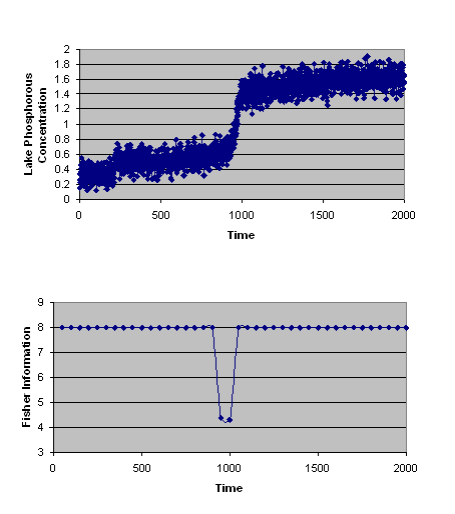
\includegraphics[width=0.8\textwidth]{fihser mts dados pouco barulho.png}
    \caption{Eutrofização de um lago com pouco barulho}
    \label{fig:Eutrofizacao de um lago com pouco barulho}
\end{figure}
\begin{figure}[H]
    \centering
    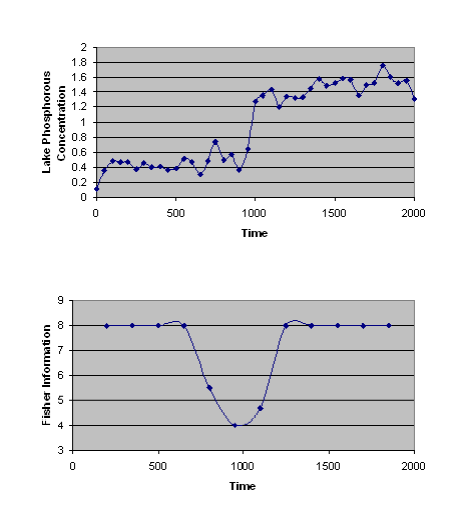
\includegraphics[width=0.8\textwidth]{fisher poucos dados baruhlo.png}
    \caption{Eutrofização de um lago com muito barulho}
    \label{fig:Eutrofizacao de um lago com muito barulho}
\end{figure}
\subsection{Conclusão}
Para o conjunto de dados reais, do estreito de bering, usaram-se 65 variaveis e fizeram a separação
entre as ambientais e as animais. Enquanto os dados são relativamente espaçados, medidos anualmente
e com muito baruhlo, ainda é possivel ver a mudança de informação de fisher, não sendo o pico
abrupto mais sim uma area de minimo  e o começo de uma queda para um flip mais recente. Não é
possivel necessariamente definir exatamente o ano do flip, talvez pelo método de calculo dele, que
foi por uma especie de convolução, mas se é possivel atribuir um intervalo a qual se tem o minimo e
atribuir o flip la. Enquanto sim é mais robusto, não precisou saber o momento exato do flip, coisa
que no artigo original eles precisavam, foi se calculado com um dataset barulhento e real de forma
bastante satisfatoria. O nivel de propagação pode ser visto mudando o nivel de restrição no calculo
(parte matematica não escrita ainda). Uma grande propagação é vista como uma queda abrupta na
informação de fisher para conjuntos de restrição baixa. Ademais, a maior queda observada no regime
de 77 do que de 89 nos diz que o de 77 foi de maior magnitude e possivelmente de maior impacto no
ecosistema. O nivel de restrição é algo que não é definido quanto para cada, depende um pouco de
teste para identificar. Uma restrição muito baixa e não vamos detectar nenhum regime, e uma muito
alta tambem não vmaos identificar. A depender do nivel de restrição tambem, não conseguimos detectar
flips de menor propagação, o que pode ser problematico.
\section{Identificações em shifts ecologicos (2008)}
\subsection{Introdução}
Enquanto tem sido um grande topico de estudos e interesse da comunidade cientifica entender, tentar
prever, identificar e analisar as mudanças de regimes ecologicos que ocorrem, interessantemente a
aplicação da estatistica não foi muito usada, apenas iniciando-se relativamente recentemente, mas
ainda extremamente restrito e muitas vezes usados em apenas certas ocasiões e muitas vezes apenas em
ecossistemas marinhos. Mas com o grande desenvolvimento da estatistica, da area de Teoria da
informação, vem se tornando cada vez mais viavel essa utilização e esse artigo visa reunir e
apresentar os principais métodos que se tinham desenvolvidos na epoca (2008), alem de mostrar suas
vantagens, problemas e possiveis coisas a serem optimizadas. \par

Em um modelo muito simplificado de ecologia, em um sistema vamos supor 2 estados, independente de
que sejam estaveis, lineares, ciclicos, caoticos, mas a mudança abrupta entre esses dois estados, ou
seja, indo do 1 para o 2 ou do 2 para o 1 identificam um shift ecologico. O grande uso da
estatistica e da matematica, sendo justo, é a identficação desses picos. Se fossemos colocar um
pulo, entre um estado ao outro, supondo, uma das coisas mais importantes na estatica de inferencia
foi a detecção desses pulos em um conjunto de dados.

\subsection{Métodos de detecção}
\begin{enumerate}
    \item O primeiro a ser considerado é apenas um tratamento e uma analise preliminar dos dados. A
    ideia principal é tentar resaltar esses pulos entre os dados para que uma analise mais simples
    consiga detectar esses flips. Um dos métodos mais usados, que é simples, facil e relativamente
    util, mas tem problemas que serão colocados depois é simplesmente achar o desvio padrão dos
    dados e fazer uma analise sobre (perguntar a mari posteriormente sobre). Esse método, simples,
    porem pode levar a falsos positivos, o que não é o desejado.
    
    \item Um outro método que é bastante utilizado, inclusive no dataset do estreito de bering, é a
    analise das componentes principais (PCA). Enquanto muito util e relativamente eficaz, detectando
    sim o shift, ela possui erros. Ela naturalmente é linear, pois acha os versores que maximizam a
    variancia do dataset, não capturando relações não lineares. Alem de que, em um sentido de
    Algebra linear, pode e vão ocorrer distorções, variando de set a set, dos dados, pois um dos
    requerimentos é a independencia linear. Alem disso, ela pode mostrar multimodalidade em datasets
    que não são, inclusive podendo apresentar para dados retirados de uma normal. enquanto util e
    bom para vizualização de dados, não é a mais certeira e eficaz
    
    \item Um método que pode ser usado é um teste de hipotese. Mais especifico, usando um método de
    intervenção pode ser usado. Mas por que colocar um teste de hipotese? Dados reais apresentam um
    alto grau de barulho, então métodos que olham para valores extremos, por exemplo, podem detectar
    um falso postivo. Com um teste de hipotese, colocando um nivel de confiança \(\alpha =5\% \),
    podemos evitar um pouco esses falsos positivos. Um dos problemas de usarmos o método de
    intervenção é que precisamos, necessariamente, saber o tempo em que ocorreu a mudança, o que
    implica estimarmos usando algum outro método. Podemos fazer um teste para cada ponto para
    sabermos se houve ou não uma mudança de regime, obtendo valores criticos, que devem ser mais
    altos que na estatistica classica. (esse finalment eu não entendi, perguntar para a mari dps.)
\end{enumerate}
\subsection{Conclusão}
Existem diversas outras formas de se explicar e mostrar as mudanças ecologicas, não so com a
informação de fisher. Algumas, não tão complexas como as outras, mas todas apresentando algum ponto
negativo sobre. A grande questão que analisei é a incerteza quanto ao tempo exato de se identificar
a mudança, sendo ela extremamente significativa ou não. Alem de que, muitas vezes se requerem muitas
variaveis e uma computação talvez um pouco intensa e complexa, então é algo a sem pensar. Num lado
mais de aprensentação, talvez uma analise visual e tentar mostrar a estatistica seja algo
interessante, já que muitos não apresentam isso.
\section{Calculando e interpretando a informação de Fisher. Um estudo de caso (2009)}
\subsection{Introdução}
Alem de seu uso na ecologia, esse artigo tambem cita o desenvolvimento da informação de fisher em
outras disciplinas, como economia, medindo a informação em uma pseudo-economia, sistemas urbanos e
ecossistemas regionais. (pesquisar mais sobre depois). Alem disso, como eu ja tinha pensado sobre,
se mostra ainda um pouco de dificuldadede no calculo da integral, necessitando de calculo, ou
estimativas, das derivadas de primeira e segunda ordem, que por si so já são trabalhosas, mas são
amplificadas pelo fato de os dados serem espaçados e com muito barulho. Alem de que ainda é de
dificil interpretação o valor que sai lá. O que extamente diz? Sua ordem de grandeza significa algo?
\subsection{Desenvolvimento, resultados e discussões.}
A solução analitica da equação de fisher é dado por
\begin{equation}
    I(t_i)=\frac{1}{T}\int_{t_i}^{t_{i+T}} \frac{(s^{\prime\prime})^{2} }{(s^\prime)^4 }
\end{equation}
onde
\begin{equation}
    s^\prime (t)=\sqrt{\sum_{i}^m(\frac{\mathrm{d}y_i}{\mathrm{d}t} )^{2} } 
\end{equation}
\begin{equation}
    s^{\prime\prime}(t)=\frac{1}{s^\prime }\sum_{i}^m\frac{\mathrm{d}y_i}{\mathrm{d}t} \frac{\mathrm{d}^{2} y_i}{\mathrm{d}t^{2}}
\end{equation}
Para casos de uma função quadratica, teriamos uma informação que vai para o infinito no seu ponto de
inflexão. Uma linear não nos da uma informação nenhuma e uma constante nos da uma informação
constante, assim como uma senoidal. Uma exponencial nos da uma informação exponencial inversa ao
valor da função. Se a exponencial da função cresce, a informação descresce e vice versa. O
interessante é a questão da periodica, pois nela, se tivermos o periodo \(T\) sua informação é
constante por todo periodo, então para uma analise ecologica o ideal é achar o periodo, pois
facilita a interpretação. Esse periodo pode ser estimado pelos métodos descritos em \ref{sec:Calculo
do periodo}. \par

A interpretação da informação pode vir direta das hipoteses citadas em \ref{hip:Hipotese dos modelos
sustentaveis}, onde se divermos sistemas em que \(\frac{\mathrm{d}I}{\mathrm{d}t} \approx 0\), eles
são considerados sustentaveis. Uma periodica, ou constante são teoricamente sustentaveis
de acordo com nossas hipoteses. Uma reta por sua vez, mesmto tendo uma baixa variação de fisher
não seria considerada sustentavel pois em qualquer instante que se mede ela, ela esta em um estado
diferente, por isso não seria sustentavel. Uma exponencial, sempre estando variando, indica um
sistema que ainda não se estabilozou e busca essa estabilidade. \par

Mesmo que um sistema seja estavel, muitas vezes ele pode estar em um estado que não interessa para
gente. Um lugar completamente deserto, onde praticamente nada vive é, em tese, sustentavel, pois a
variação da informação de fisher tende a zero. Mas é algo desejavel para nos? Tudo está na
interpretação e as vezes não necessariamente é algo completamente indesejavel perder informação de
fisher, desde que essa perca nos leve a algo que seja ecologico. O grande jogo esta na analise da
derivada da informação. \par

Fazer depois
\end{document}